% Journal of Astrophysics and Astronomy: official double-column class (jaa.cls) and reference style (apj.bst),
% both from the journal's author kit (JAA.zip).
\documentclass{jaa}
\usepackage{natbib}
\bibliographystyle{apj}
\usepackage{graphicx}
\usepackage{amssymb}
\usepackage{booktabs}
\usepackage{xcolor}
\usepackage{textcomp}
\usepackage{url}
\usepackage[colorlinks=true,linkcolor=blue,citecolor=blue,urlcolor=blue]{hyperref}

% Every result number below is a macro generated from committed result files
% (research/figures/paper_main.py and research/figures/phase4_numbers.py).
% GENERATED by research/figures/paper_main.py -- do not edit
\newcommand{\CausalBugPct}{98\%}
\newcommand{\SimGamma}{0.1}
\newcommand{\SimLengthscale}{1.2}
\newcommand{\SimNEvents}{1000}
\newcommand{\SimNModeled}{587}
\newcommand{\SimNWithheld}{413}
\newcommand{\SimHOneVerdict}{\textbf{fail}}
\newcommand{\SimHTwoVerdict}{\textbf{pass}}
\newcommand{\SimHThreeVerdict}{\textbf{pass}}
\newcommand{\SimTtiP}{23.0\,h}
\newcommand{\SimIdP}{99\%}
\newcommand{\SimTtiBzero}{$>$\,budget}
\newcommand{\SimIdBzero}{48\%}
\newcommand{\SimHolmBzero}{$<10^{-4}$}
\newcommand{\SimRbcBzero}{0.52}
\newcommand{\SimFasterBzero}{50\%}
\newcommand{\SimSlowerBzero}{48\%}
\newcommand{\SimTtiBone}{12.05\,d}
\newcommand{\SimIdBone}{61\%}
\newcommand{\SimHolmBone}{$<10^{-4}$}
\newcommand{\SimRbcBone}{0.63}
\newcommand{\SimFasterBone}{62\%}
\newcommand{\SimSlowerBone}{27\%}
\newcommand{\SimTtiBtwo}{13.8\,h}
\newcommand{\SimIdBtwo}{72\%}
\newcommand{\SimHolmBtwo}{0.00019}
\newcommand{\SimRbcBtwo}{0.19}
\newcommand{\SimFasterBtwo}{30\%}
\newcommand{\SimSlowerBtwo}{49\%}
\newcommand{\SimTtiBthree}{1.59\,d}
\newcommand{\SimIdBthree}{99\%}
\newcommand{\SimHolmBthree}{$<10^{-4}$}
\newcommand{\SimRbcBthree}{0.33}
\newcommand{\SimFasterBthree}{48\%}
\newcommand{\SimSlowerBthree}{25\%}
\newcommand{\SimObsP}{4.2}
\newcommand{\SimObsBthree}{2.9}
\newcommand{\SimHtwoFast}{0.414}
\newcommand{\SimHtwoSlow}{0.152}
\newcommand{\SimHtwoEst}{0.261}
\newcommand{\SimHtwoCI}{[0.153, 0.368]}
\newcommand{\SimHtwoFastCI}{[0.314, 0.514]}
\newcommand{\SimHtwoSlowCI}{[0.113, 0.195]}
\newcommand{\SimTprP}{96\%}
\newcommand{\SimTprBthree}{21\%}
\newcommand{\SimHthreeEst}{76}
\newcommand{\SimHthreeCI}{[66, 84]}
\newcommand{\SimAucP}{0.993}
\newcommand{\SimAucBthree}{0.666}
\newcommand{\SimAucBtwo}{0.696}
\newcommand{\SimAucPown}{0.714}
\newcommand{\SimTprPown}{21\%}
\newcommand{\SimCwWhBthree}{97\%}
\newcommand{\SimCwWhP}{6\%}
\newcommand{\SimAccModP}{100\%}
\newcommand{\SimAccModBthree}{100\%}
\newcommand{\SimFaP}{0\%}
\newcommand{\SimFaPModelError}{13\%}
\newcommand{\SimAccModPModelError}{87\%}
\newcommand{\SimAucPModelError}{0.891}
\newcommand{\SimAucBthreeModelError}{0.706}
\newcommand{\SimAucPCrowding}{0.975}
\newcommand{\SimObsAllP}{4.2}
\newcommand{\SimAccModPAll}{100\%}
\newcommand{\SimCwWhPAll}{6\%}
\newcommand{\SimFlagP}{89\%}
\newcommand{\SimAucAblP}{0.993}
\newcommand{\SimObsAllNoDecay}{3.6}
\newcommand{\SimAccModNoDecayAll}{99\%}
\newcommand{\SimCwWhNoDecayAll}{31\%}
\newcommand{\SimFlagNoDecay}{65\%}
\newcommand{\SimAucAblNoDecay}{0.936}
\newcommand{\SimObsAllNoAdeq}{4.3}
\newcommand{\SimAccModNoAdeqAll}{100\%}
\newcommand{\SimCwWhNoAdeqAll}{6\%}
\newcommand{\SimFlagNoAdeq}{89\%}
\newcommand{\SimAucAblNoAdeq}{0.992}
\newcommand{\SimObsAllBthree}{2.8}
\newcommand{\SimAccModBthreeAll}{100\%}
\newcommand{\SimCwWhBthreeAll}{97\%}
\newcommand{\SimObsAllBtwo}{4.9}
\newcommand{\SimAccModBtwoAll}{88\%}
\newcommand{\SimCwWhBtwoAll}{69\%}
\newcommand{\SimObsAllBone}{3.2}
\newcommand{\SimAccModBoneAll}{80\%}
\newcommand{\SimCwWhBoneAll}{75\%}
\newcommand{\SimObsAllBzero}{5.0}
\newcommand{\SimAccModBzeroAll}{79\%}
\newcommand{\SimCwWhBzeroAll}{1\%}
\newcommand{\SimDeltaKilonova}{1.59}
\newcommand{\SimDeltaShock}{0.32}
\newcommand{\SimDeltaFlare}{-0.56}
\newcommand{\SimDeltaGrb}{0.15}
\newcommand{\SimHtwoModelErrorEst}{-0.098}
\newcommand{\SimHtwoModelErrorCI}{[-0.171, -0.024]}
\newcommand{\SimHtwoCrowdingEst}{0.232}
\newcommand{\SimHthreeModelErrorEst}{17}
\newcommand{\SimHthreeModelErrorCI}{[8, 31]}
\newcommand{\SimAccModBthreeModelError}{99\%}
\newcommand{\SimHOneCrowding}{fail}
\newcommand{\SimHTwoCrowding}{pass}
\newcommand{\SimHThreeCrowding}{pass}
\newcommand{\SimHOneModelError}{fail}
\newcommand{\SimHTwoModelError}{fail}
\newcommand{\SimHThreeModelError}{pass}
\newcommand{\RealCHOneVerdict}{\textbf{pass}}
\newcommand{\RealCHTwoVerdict}{\textbf{pass}}
\newcommand{\RealCHThreeVerdict}{\textbf{pass}}
\newcommand{\RealCHFourVerdict}{\textbf{pass}}
\newcommand{\RealCHFiveVerdict}{\textbf{fail}}
\newcommand{\RealRHOneVerdict}{\textbf{pass}}
\newcommand{\RealRHTwoVerdict}{\textbf{pass}}
\newcommand{\RealRHThreeVerdict}{\textbf{fail}}
\newcommand{\RealRHFourVerdict}{\textbf{pass}}
\newcommand{\RealRHFiveVerdict}{\textbf{fail}}
\newcommand{\RealNEvents}{364}
\newcommand{\RealNWithheld}{88}
\newcommand{\RealNModeled}{276}
\newcommand{\RealCAuc}{0.79--0.81}
\newcommand{\RealCCwWhBthree}{50--56\%}
\newcommand{\RealCAccModBthree}{58--62\%}
\newcommand{\RealCCwWhP}{7--14\%}
\newcommand{\RealCAccModP}{59--63\%}
\newcommand{\RealCCwWhBone}{40--45\%}
\newcommand{\RealCAccModBone}{54--56\%}
\newcommand{\RealCFlagP}{39--47\%}
\newcommand{\RealCFaP}{8\%}
\newcommand{\RealRAuc}{0.77--0.80}
\newcommand{\RealRCwWhBthree}{78--80\%}
\newcommand{\RealRAccModBthree}{59--62\%}
\newcommand{\RealRCwWhP}{12--19\%}
\newcommand{\RealRAccModP}{53--54\%}
\newcommand{\RealRCwWhBone}{48--49\%}
\newcommand{\RealRAccModBone}{51--55\%}
\newcommand{\RealRFlagP}{64--73\%}
\newcommand{\RealRFaP}{24--25\%}
\newcommand{\RealCObsP}{2.3}
\newcommand{\RealCObsBthree}{2.6}
\newcommand{\RealCObsBzero}{5.0}
\newcommand{\RealRObsP}{5.0}
\newcommand{\RealRObsBthree}{5.0}
\newcommand{\RealRObsBzero}{5.0}
\newcommand{\ConfAlpha}{0.1}
\newcommand{\ConfAlphaPct}{10\%}
\newcommand{\ConfLambda}{0.25}
\newcommand{\ConfNFresh}{489}
\newcommand{\ConfNCal}{456}
\newcommand{\ConfHCOneVerdict}{\textbf{pass}}
\newcommand{\ConfHCTwoVerdict}{\textbf{pass}}
\newcommand{\ConfHCThreeVerdict}{\textbf{pass}}
\newcommand{\ConfHCFourVerdict}{\textbf{pass}}
\newcommand{\ConfHCFiveVerdict}{\textbf{pass}}
\newcommand{\ConfHCSixVerdict}{\textbf{fail}}
\newcommand{\ConfFa}{3--6\%}
\newcommand{\ConfAccGain}{6--8~points}
\newcommand{\ConfFlag}{42--55\%}
\newcommand{\ConfAucGain}{+0.012--+0.039}
\newcommand{\ConfAccFreshCL}{66--69\%}
\newcommand{\ConfAccFreshP}{61--66\%}
\newcommand{\ConfAccFreshBthree}{60\%}
\newcommand{\ConfAccFreshBthreeConf}{57--58\%}
\newcommand{\ConfRawFaFreshP}{7--9\%}
\newcommand{\ConfCwUnkCL}{26--32\%}
\newcommand{\ConfCwUnkP}{7--14\%}
\newcommand{\ConfCwUnkBthree}{50--56\%}
\newcommand{\ConfFlagBthreeConf}{41--52\%}
\newcommand{\ConfObsP}{2.3--2.4}
\newcommand{\ConfObsL}{3.1--3.2}

% GENERATED by research/figures/phase4_numbers.py -- do not edit
\newcommand{\FleetNEpisodes}{250}
\newcommand{\FleetNEvents}{1000}
\newcommand{\FleetNModeled}{592}
\newcommand{\FleetNUnknown}{408}
\newcommand{\FleetReserveA}{10}
\newcommand{\FleetReserveG}{3}
\newcommand{\FleetReserveK}{10}
\newcommand{\FleetReserveO}{1}
\newcommand{\FleetHFourOneVerdict}{\textbf{pass}}
\newcommand{\FleetHFourOneEst}{+10.5}
\newcommand{\FleetHFourOneCI}{[+6.3, +14.5]}
\newcommand{\FleetHFourTwoVerdict}{\textbf{fail}}
\newcommand{\FleetHFourTwoEst}{-1.5}
\newcommand{\FleetHFourTwoCI}{[-5.4, +2.3]}
\newcommand{\FleetHFourThreeVerdict}{\textbf{pass}}
\newcommand{\FleetHFourThreeEst}{+12.0}
\newcommand{\FleetHFourThreeCI}{[+8.2, +15.8]}
\newcommand{\FleetHFourFourVerdict}{\textbf{pass}}
\newcommand{\FleetHFourFourEst}{+0.5}
\newcommand{\FleetHFourFourCI}{[-1.8, +2.8]}
\newcommand{\FleetHEOneVerdict}{\textbf{pass}}
\newcommand{\FleetHETwoVerdict}{\textbf{pass}}
\newcommand{\FleetHEOneMaxK}{1}
\newcommand{\FleetHEOneN}{592}
\newcommand{\FleetHEOneMaxUpper}{0.008}
\newcommand{\FleetHETwoK}{0}
\newcommand{\FleetHETwoN}{4736}
\newcommand{\FleetAccO}{87\%}
\newcommand{\FleetObsO}{5.1}
\newcommand{\FleetLsO}{-0.80}
\newcommand{\FleetAucO}{0.93}
\newcommand{\FleetCwUO}{8\%}
\newcommand{\FleetFlagO}{48\%}
\newcommand{\FleetEDetO}{26\%}
\newcommand{\FleetStaleO}{0\%}
\newcommand{\FleetDupO}{2.3}
\newcommand{\FleetAccG}{76\%}
\newcommand{\FleetObsG}{5.4}
\newcommand{\FleetLsG}{-0.99}
\newcommand{\FleetAucG}{0.88}
\newcommand{\FleetCwUG}{4\%}
\newcommand{\FleetFlagG}{39\%}
\newcommand{\FleetEDetG}{16\%}
\newcommand{\FleetStaleG}{88\%}
\newcommand{\FleetDupG}{2.0}
\newcommand{\FleetAccA}{75\%}
\newcommand{\FleetObsA}{3.7}
\newcommand{\FleetLsA}{-0.88}
\newcommand{\FleetAucA}{0.90}
\newcommand{\FleetCwUA}{0\%}
\newcommand{\FleetFlagA}{45\%}
\newcommand{\FleetEDetA}{21\%}
\newcommand{\FleetStaleA}{29\%}
\newcommand{\FleetDupA}{1.3}
\newcommand{\FleetAccK}{74\%}
\newcommand{\FleetObsK}{3.8}
\newcommand{\FleetLsK}{-0.91}
\newcommand{\FleetAucK}{0.89}
\newcommand{\FleetCwUK}{0\%}
\newcommand{\FleetFlagK}{42\%}
\newcommand{\FleetEDetK}{19\%}
\newcommand{\FleetStaleK}{29\%}
\newcommand{\FleetDupK}{1.4}
\newcommand{\FleetAccAOne}{72\%}
\newcommand{\FleetObsAOne}{3.8}
\newcommand{\FleetLsAOne}{-0.95}
\newcommand{\FleetAucAOne}{0.88}
\newcommand{\FleetCwUAOne}{1\%}
\newcommand{\FleetFlagAOne}{39\%}
\newcommand{\FleetEDetAOne}{14\%}
\newcommand{\FleetStaleAOne}{45\%}
\newcommand{\FleetDupAOne}{1.2}
\newcommand{\FleetLinkUpOne}{1\%}
\newcommand{\FleetLinkUpFive}{12\%}
\newcommand{\FleetMEFalseUnknownO}{14\%}
\newcommand{\FleetMEFalseUnknownG}{5\%}
\newcommand{\FleetExAminusGEst}{+2.4}
\newcommand{\FleetExAminusGCI}{[-1.0, +5.6]}
\newcommand{\FleetExOminusGEst}{+5.1}
\newcommand{\FleetExOminusGCI}{[+1.0, +9.1]}
\newcommand{\FleetExOminusAEst}{+2.7}
\newcommand{\FleetExOminusACI}{[-0.7, +6.2]}
\newcommand{\FleetExAminusKEst}{-0.5}
\newcommand{\FleetExAminusKCI}{[-3.0, +1.9]}
\newcommand{\FleetExAccO}{81\%}
\newcommand{\FleetBOneVerdict}{\textbf{pass}}
\newcommand{\FleetBOneEst}{+5.3}
\newcommand{\FleetBOneCI}{[+2.9, +7.6]}
\newcommand{\FleetBOneMag}{5.3}
\newcommand{\FleetBTwoVerdict}{\textbf{pass}}
\newcommand{\FleetBTwoEst}{-1.3}
\newcommand{\FleetBTwoCI}{[-3.0, +0.5]}
\newcommand{\FleetBTwoMag}{1.3}
\newcommand{\FleetBThreeVerdict}{\textbf{pass}}
\newcommand{\FleetBThreeEst}{+7.9}
\newcommand{\FleetBThreeCI}{[+5.9, +9.8]}
\newcommand{\FleetBThreeMag}{7.9}
\newcommand{\FleetBFourVerdict}{\textbf{pass}}
\newcommand{\FleetBFourEst}{+9.4}
\newcommand{\FleetBFourCI}{[+6.9, +12.0]}
\newcommand{\FleetBFourMag}{9.4}
\newcommand{\FleetHFourOneMag}{10.5}
\newcommand{\FleetBFiveVerdict}{\textbf{pass}}
\newcommand{\FleetBFiveEst}{+0.27}
\newcommand{\FleetBFiveCI}{[+0.23, +0.31]}
\newcommand{\FleetBDenseAGEst}{+1.8}
\newcommand{\FleetBDenseAGCI}{[-0.8, +4.4]}
\newcommand{\FleetBNEvents}{2000}
\newcommand{\FleetDenseLinkUpOne}{9\%}
\newcommand{\FleetDenseLinkUpFive}{38\%}
\newcommand{\FleetBAccOSparse}{80\%}
\newcommand{\FleetBAccODense}{70\%}
\newcommand{\ECalFa}{3.9--5.0\%}
\newcommand{\ECalN}{456}
\newcommand{\EHROneVerdict}{\textbf{pass}}
\newcommand{\EHRTwoVerdict}{\textbf{pass}}
\newcommand{\EFreshN}{489}
\newcommand{\EWithheldN}{88}
\newcommand{\EFreshFa}{3.3--4.3\%}
\newcommand{\EFreshFaUpper}{6.1\%}
\newcommand{\EDet}{26--31\%}
\newcommand{\EDetLower}{19\%}
\newcommand{\EDetBthree}{36--41\%}
\newcommand{\EFreshFaBthree}{5.1--6.1\%}
\newcommand{\EDetL}{40--50\%}


\makeatletter
% Plain page numbers only. The journal fills its own header (volume, year, article id, DOI) after acceptance.
\def\ps@myheadings{\let\@oddhead\@empty\let\@evenhead\@empty\def\@oddfoot{\hfil\thepage\hfil}\let\@evenfoot\@oddfoot}
\def\ps@firstpage{\let\@oddhead\@empty\let\@evenhead\@empty\def\@oddfoot{\hfil\thepage\hfil}\let\@evenfoot\@oddfoot}
\pagestyle{myheadings}
\makeatother

\begin{document}\sloppy

\title{Knowing What You Do Not Know: Open-World Follow-Up\\ Planning for Fading Transients, from One Spacecraft to a Fleet}

\author{Dr.~Smitha Shekar B\textsuperscript{2}, Dr.~Harish G\textsuperscript{2}, Joyce Malik\textsuperscript{1,*}, Anup H\textsuperscript{1}, Moghitha B\textsuperscript{1} and Swathi Sathish\textsuperscript{1}}
\affilOne{\textsuperscript{1}School of Computer Science and Engineering Program, Dr.\ Ambedkar Institute of Technology, Outer Ring Road, Mallathahalli, Bengaluru 560056, Karnataka, India.}
\affilTwo{\par\vspace{4pt}\textsuperscript{2}Professor, Computer Science and Engineering Program, Dr.\ Ambedkar Institute of Technology, Bengaluru 560056, Karnataka, India.}

\twocolumn[{

\maketitle
\vspace{10pt}

\corres{joycemalik14@gmail.com (ORCID 0009-0001-8293-8064). Co-authors: alexanubius6808@gmail.com (A.H.), moghithab4@gmail.com (M.B.), sathishswathi04@gmail.com (S.S.)}
\vspace{8pt}

\begin{abstract}
Sky surveys find more short-lived explosions than any telescope can follow, so future spacecraft will have to decide what to measure next. Today's planners choose the measurement that best separates the object types they already know. But when something new appears, they have no way to say so, and every extra measurement makes them more sure of a wrong answer. We give the planner one more option, ``none of the above'', and let it measure only forward in time, as a real spacecraft must. In simulation it recognised \SimTprP\ of never-seen object types at a 5\% false-alarm rate, against \SimTprBthree\ for the usual approach. On \RealNEvents\ real transients from the Zwicky Transient Facility, it was confidently wrong about \RealCCwWhP\ of the unfamiliar objects, against \RealCCwWhBthree. We then give the word ``unknown'' a false-alarm guarantee that holds at every step, and spread the planner over satellites that can only talk when they see each other. Sharing observations helped, but where the satellites sit mattered more, and a well-connected fleet in one orbital plane was \FleetBFourMag\ percentage points less accurate than a spread one.
\end{abstract}

\keywords{transient follow-up---open-set recognition---Bayesian experimental design---anytime-valid inference---distributed spacecraft autonomy---preregistration.}

}]

\section{Introduction}\label{sec:intro}

Wide-field surveys now find far more transients than any follow-up programme can observe \citep{Bellm2019,Ivezic2019}. Many of these events fade within hours, so the measurements that would separate one explanation from another are only available for a short time. Choosing the next measurement is therefore a planning problem. The standard way to plan it is to pick the measurement with the highest expected information gain (EIG) about the event's class \citep{Lindley1956,Chaloner1995}.

EIG is good at telling known classes apart. It cannot tell us when an event belongs to none of them. A posterior over $K$ known classes always sums to one, so when a genuinely new object comes in, every new measurement pushes the planner further towards whichever known class fits least badly. The planner becomes more confident exactly when it should become less confident. The problem sits in the hypothesis space itself, so tuning will not fix it. A threshold on closed-world uncertainty fails for the same reason, since a confident wrong answer has low entropy.

We start from this observation and ask four questions. For each one, the hypotheses were committed before the test data were run.
\begin{enumerate}
\item Does adding an explicit unmodelled hypothesis $h_0$ to the planner stop it from confidently misclassifying unknown events, and what does that cost on known ones? We test this in simulation (Sect.~\ref{sec:sim}) and on real ZTF events (Sect.~\ref{sec:real}).
\item Can the ``unknown'' decision come with a guaranteed false-alarm rate? We try a conformal threshold (Sect.~\ref{sec:conf}) and anytime-valid e-values (Sect.~\ref{sec:fleet}).
\item How does respecting the order of time change these conclusions? (Sect.~\ref{sec:disc})
\item When the planner runs on a fleet whose spacecraft can only talk while in line of sight, how much does communication help, and does coordinating plans add anything beyond sharing data? (Sect.~\ref{sec:fleet})
\end{enumerate}

Our main findings and contributions are:
\begin{itemize}
\item In simulation and on real events, the open-world posterior is the part that matters. An extra utility term aimed at testing $h_0$ adds nothing.
\item We give two ways to attach a guarantee to ``unknown''. The first is a split-conformal threshold. The second, new here, is a universal-inference e-process. It is valid at every step, needs no calibration data, and can be combined across spacecraft by simple averaging.
\item We measure how a causal time order changes the conclusions of follow-up studies.
\item We build a decentralised fleet that shares observations as conflict-free replicated data types (CRDTs), and we measure what communication and coordination are worth under real link geometry.
\end{itemize}

\section{Related work and the gap}\label{sec:related}

\paragraph{Anomaly and out-of-taxonomy detection.} Broker-level systems rank alerts by how unusual they look. They use deep embeddings with isolation forests \citep{Villar2021}, real-time similarity search \citep{Aleo2024}, autoencoders on the ZTF stream \citep{Iskandarli2026}, active anomaly detection in Fink \citep{Pruzhinskaya2026} and classifier-based multi-class anomaly scores \citep{Gupta2024}. FLARE runs out-of-taxonomy detection in production \citep{Sasli2026FLARE} and reports that blind detection recovers few out-of-taxonomy objects at a 1\% false-alarm rate. ASTRANet adds conformal calibration to spectroscopic classification \citep{Sasli2026ASTRANet}. All of these work on data that already exist, so none of them decides which measurement to take next to make the unknown recognisable.

\paragraph{Information-driven follow-up.} Information-theoretic and active-learning methods choose which objects deserve a spectrum \citep{Astudillo2020,Kennamer2020,Moller2025}, and multi-telescope schedulers optimise tiling and cadence \citep{Coughlin2019,Almualla2021}. They work in a closed world, and at the level of targets rather than the individual measurements of one event.

\paragraph{Experimental design under misspecification.} Bayesian design has been made robust to outliers and to a wrong noise model \citep{Barlas2025,Catanach2023}, and it has been extended to learn model discrepancy \citep{Yang2025}. Amortised policies make it non-myopic \citep{Foster2021,Hedman2025}. None of these includes an explicit ``none of the above'' hypothesis or a deadline. Conformal methods for unseen classes exist in general form \citep{Xie2025}, but not for sequential decisions.

\paragraph{Distributed spacecraft.} Consensus auctions \citep{Choi2009,Perone2026}, dynamic distributed constraint optimisation \citep{Zilberstein2026} and flight demonstrations \citep{Adams2024} allocate fixed requests over limited links. Our setting is harder in one specific way. The value of a measurement depends on a belief about what the event is, and that belief is itself spread across spacecraft and often out of date. Decentralised information gathering in robotics \citep{Atanasov2015} is the closest in spirit, but it is closed-world.

\paragraph{The gap.} To our knowledge, no earlier study puts an explicit unmodelled hypothesis inside a sequential, causal, multi-spacecraft measurement planner, and then tests it against preregistered hypotheses on real unknown transients with a certified false-alarm rate. This is the gap we fill, and we keep our claim limited to it.

\section{Method}\label{sec:method}

\paragraph{Belief.} For $K$ modelled classes with forward models $f_k(t;A)$, the planner keeps an exact grid posterior over the class $k$ and the amplitude $A$. Measurements are Gaussian, $y\sim\mathcal N(f_k(t;A),\sigma_i^2)$, where $\sigma_i$ comes from the instrument's limiting magnitude. The open-world posterior adds one more hypothesis, $h_0$, scored by the marginal likelihood of a zero-mean Gaussian process (GP), with a uniform prior over $\{1,\dots,K,h_0\}$. $h_0$ is not a new physical class. It simply says that none of the modelled classes explains the data.

\paragraph{Utility and causality.} A candidate action is an (epoch, spacecraft) pair that is visible and strictly later than the last measurement, so the planner can only ever measure forward in time. The planner P maximises
\begin{equation}
U(a) = I(H_{1:K};Y_a) + \beta\, I(Z;Y_a) + \gamma\, D(a),
\label{eq:utility}
\end{equation}
where $I(H_{1:K};Y_a)$ is the closed-world class EIG, $Z=\mathbb 1[h_0]$, and $D(a)$ is a Fisher-information proxy for what we lose by waiting until the same spacecraft's next opportunity. We compare against a fixed cadence (B0), the constellation's original auction score with no belief (B1), classifier-entropy sampling (B2) and closed-world EIG (B3). The ablations remove $\gamma$ or $\beta$.

\paragraph{Two guarantees for ``unknown''.} The conformal rule flags ``unknown'' when $s=\log p(D\mid h_0)-\max_c\log p(D\mid c)$ goes above a split-conformal threshold calibrated per known class \citep{Vovk2005,Angelopoulos2023}. Its guarantee holds at the end of the measurement budget, and it needs exchangeable calibration events. The e-process rule needs neither. Once we fix the GP as the alternative, universal inference \citep{Wasserman2020} gives
\begin{equation}
E_t=\frac{p_{\rm GP}(D_t)}{\sup_{c,A}L(c,A;D_t)},\qquad P\Big(\sup_t E_t\ge 1/\alpha\Big)\le\alpha
\label{eq:eprocess}
\end{equation}
under any modelled class, by Ville's inequality \citep{Ramdas2023}. This holds even though every measurement was chosen adaptively from earlier data. Every $f_k$ is linear in $A$, so the supremum is exact. There is a price for needing no calibration, though: the guarantee holds only if the templates and the noise model are right.

\paragraph{From one planner to a fleet.} Each spacecraft keeps a grow-only set of observation records (a G-Set CRDT, \citealp{Shapiro2011}). Merging two sets is just their union, so a record that arrives twice or out of order is never counted twice, and the belief is a deterministic function of the set. Two spacecraft can exchange records only when they are within range $R$ and their line of sight clears the Earth plus 80\,km. We check this from real orbital elements every two minutes, and information spreads by store-and-forward. At each epoch, the spacecraft in each connected component run a sequential greedy auction on P's utility. They add ``believer'' pseudo-observations at the predictive mean, so a second bid on the same event sees diminishing returns \citep{Ginsbourger2010}. A spacecraft spends a measurement only if its utility is above a reserve price. On board, a spacecraft can combine ``unknown'' evidence by averaging the last e-values it has heard, and the average is still an e-value under any dependence \citep{VovkWang2021}.

\section{What we tested}\label{sec:tests}
We ran four studies, and before each test we wrote down what we expected and how it would count as a pass. Table~\ref{tab:tests} lists every prediction and what happened, failures included. The rest of the paper tells the story behind it, so the text keeps to the numbers that matter and leaves intervals and per-seed detail to the tables.

\begin{table*}[t]
\centering\footnotesize
\caption{Every preregistered prediction, in plain words, and its outcome on the sealed test data.}
\label{tab:tests}
\begin{tabular}{llc@{\hskip 18pt}llc}
\toprule
& Prediction & Outcome & & Prediction & Outcome\\
\midrule
\multicolumn{3}{l}{\textit{Study 1: simulation}} & \multicolumn{3}{l}{\textit{Study 4: a fleet of eight satellites}}\\
H1 & P identifies known events fastest & \SimHOneVerdict & H4.1 & Ideal links beat no links & \FleetHFourOneVerdict\\
H2 & Urgency matters more for fast events & \SimHTwoVerdict & H4.2 & Realistic links beat no links & \FleetHFourTwoVerdict\\
H3 & ``None of the above'' finds new types & \SimHThreeVerdict & H4.3 & Ideal links beat realistic links & \FleetHFourThreeVerdict\\
\multicolumn{3}{l}{\textit{Study 2: real ZTF events}} & H4.4 & Coordinating plans adds little & \FleetHFourFourVerdict\\
H1 & Fewer confident errors on unknowns & \RealCHOneVerdict & HE1 & Few false alarms per spacecraft & \FleetHEOneVerdict\\
H2 & Unknowns rank above supernovae & \RealCHTwoVerdict & HE2 & Few false alarms when combined & \FleetHETwoVerdict\\
H3 & No more confident errors on supernovae & \RealCHThreeVerdict & B1 & Realistic links help at equal spending & \FleetBOneVerdict\\
H4 & Colour helps & \RealCHFourVerdict & B2 & Coordinating plans adds little & \FleetBTwoVerdict\\
H5 & Supernova accuracy within 5 points & \RealCHFiveVerdict & B3 & When to spend matters & \FleetBThreeVerdict\\
\multicolumn{3}{l}{\textit{Study 3: guaranteed false-alarm rate}} & B4 & A spread fleet beats one plane & \FleetBFourVerdict\\
HC1 & False alarms within 10\% & \ConfHCOneVerdict & B5 & It measures at more distinct times & \FleetBFiveVerdict\\
HC2 & More accurate than closed-world & \ConfHCTwoVerdict & \multicolumn{3}{l}{\textit{Study 3, continued: a guarantee with no calibration}}\\
HC3 & No more confident errors & \ConfHCThreeVerdict & HR1 & False alarms within 10\% on real supernovae & \EHROneVerdict\\
HC4 & Fewer confident errors on unknowns & \ConfHCFourVerdict & HR2 & Catches real unknowns & \EHRTwoVerdict\\
HC5 & Flags real unknowns & \ConfHCFiveVerdict & & & \\
HC6 & Lookahead ranks unknowns better & \ConfHCSixVerdict & & & \\
\bottomrule
\end{tabular}
\end{table*}

\section{Study 1: simulation}\label{sec:sim}
\paragraph{Setup.} Events come from four known classes (kilonova, shock cooling, GRB afterglow and M-dwarf flare) and three types no planner ever sees: an AT2018cow-like fast blue transient, a tidal disruption event and a deliberately unphysical oscillation. Eight Starlink satellites on real orbits watch the sky, each sees a target only when the Earth is not in the way, and every planner gets five measurements over 20 days. Table~\ref{tab:sim} gives the full results for every planner.

\paragraph{Naming the unknown is what works.} When we let the planner say ``none of the above'', it found \SimTprP\ of the never-seen event types at a 5\% false-alarm rate. The usual alternative, a threshold on how uncertain a closed-world planner is, found only \SimTprBthree\ (Fig.~\ref{fig:rocsim}). Without that extra option, closed-world information gain was confidently wrong on \SimCwWhBthreeAll\ of the unknown events, against \SimCwWhPAll\ for our planner P. It paid nothing for this on ordinary events, and kept the same accuracy on the known classes (\SimAccModPAll). We then checked whether P's gain comes from where it chooses to measure. It does not, since an uncertainty threshold computed on P's own measurements still reached an AUROC of only \SimAucPown, against \SimAucP\ for $P(h_0)$. So the gain comes from having a name for the unknown, not from clever measurement.

\begin{figure}[t]
\centering
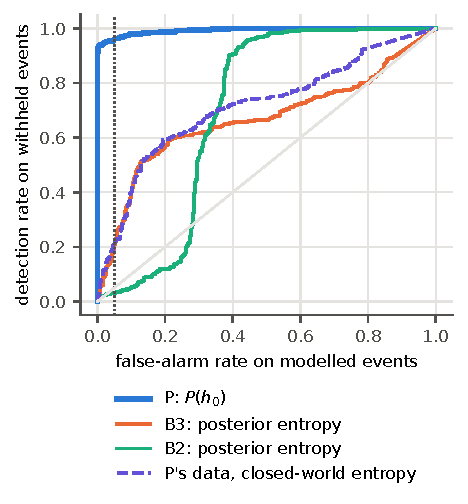
\includegraphics[width=\columnwidth]{fig3_roc_sim.pdf}
\caption{Simulation. How well each method separates never-seen event types from known ones. The dotted line marks the 5\% false-alarm point we fixed in advance.}
\label{fig:rocsim}
\end{figure}

\paragraph{It is not the fastest.} We expected P to identify known events sooner than every baseline, and it did not. A cheap rule that measures where classifiers disagree got there first on the events it could identify (median \SimTtiBtwo\ against \SimTtiP), but it gave up on many of them, identifying only \SimIdBtwo\ of events against \SimIdP\ for P (Fig.~\ref{fig:tti}).

\begin{figure}[t]
\centering
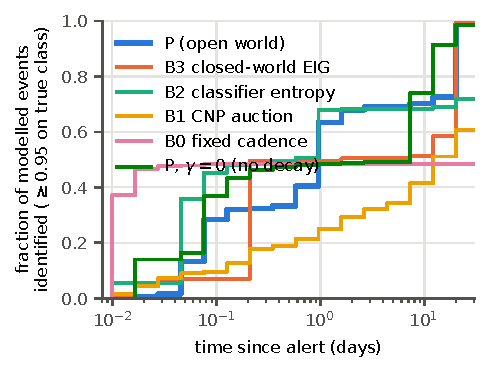
\includegraphics[width=\columnwidth]{fig1_tti.pdf}
\caption{Simulation. Share of known events identified (posterior on the true class at least 0.95) against time since the alert. The disagreement rule B2 is quickest on the events it can identify, while P identifies almost all of them, a little later.}
\label{fig:tti}
\end{figure}

\paragraph{Urgency helps fast events, but not all of them.} The decay term is meant to make the planner measure fast events before they fade. It did recover more information on kilonovae (\SimDeltaKilonova) and shock cooling (\SimDeltaShock) than on the slow GRB afterglow, but for the fastest class, the M-dwarf flare, it lost information (\SimDeltaFlare; Fig.~\ref{fig:decay}), and it reversed under model error. Its clearest benefit was indirect. Without it, the planner spent its measurements too early (\SimObsAllNoDecay\ instead of \SimObsAllP), which left $h_0$ too little data and raised confident errors on unknowns to \SimCwWhNoDecayAll. The term built to test $h_0$ directly ($\beta$) changed nothing we could measure.

\begin{figure}[t]
\centering
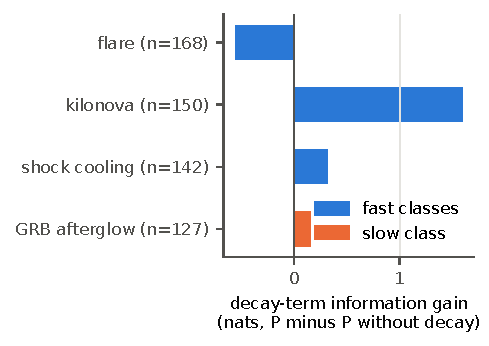
\includegraphics[width=\columnwidth]{fig2_decay.pdf}
\caption{Simulation. Information about each event's brightness gained from the decay term (P minus P without it). It helps kilonovae and shock cooling, does little for the slow class, and hurts flares.}
\label{fig:decay}
\end{figure}

\begin{table*}[t]
\centering\scriptsize
\caption{Simulation test results (1000 events per scenario). Acc.\ mod.: accuracy on modelled events (\%). CW: confident-wrong rate (\%) on unmodelled (withheld) and modelled events. $\bar n_{\rm obs}$: measurements used, out of 5. Log score: mean log probability of the true outcome (closed-world strategies cannot express ``withheld'', so they are floored at $10^{-6}$).}
\label{tab:sim}
\begin{tabular}{llrrrrr}
\toprule
Scenario & Strategy & Acc.\ mod. & CW unmod. & CW mod. & $\bar n_{\rm obs}$ & log score \\
\midrule
Nominal & P (open world) & 100 & 6 & 0 & 4.2 & -0.19 \\
 & B3 closed-world EIG & 100 & 97 & 0 & 2.8 & -5.71 \\
 & B2 classifier entropy & 88 & 69 & 0 & 4.9 & -5.82 \\
 & B1 CNP auction & 80 & 75 & 0 & 3.2 & -5.92 \\
 & B0 fixed cadence & 79 & 1 & 0 & 5.0 & -5.92 \\
 & P, $\gamma=0$ (no decay) & 99 & 31 & 0 & 3.6 & -0.87 \\
 & P, $\beta=0$ (no adequacy) & 100 & 6 & 0 & 4.3 & -0.20 \\
\midrule
Crowding & P (open world) & 99 & 14 & 0 & 4.0 & -0.43 \\
 & B3 closed-world EIG & 100 & 94 & 0 & 3.0 & -5.82 \\
 & B2 classifier entropy & 94 & 80 & 0 & 4.8 & -5.88 \\
 & B1 CNP auction & 86 & 71 & 0 & 3.1 & -5.97 \\
 & B0 fixed cadence & 76 & 1 & 0 & 5.0 & -6.03 \\
 & P, $\gamma=0$ (no decay) & 100 & 31 & 0 & 3.4 & -0.96 \\
 & P, $\beta=0$ (no adequacy) & 99 & 14 & 0 & 4.1 & -0.43 \\
\midrule
Model error & P (open world) & 87 & 21 & 8 & 3.9 & -1.21 \\
 & B3 closed-world EIG & 99 & 96 & 1 & 2.9 & -6.11 \\
 & B2 classifier entropy & 81 & 29 & 4 & 5.0 & -6.32 \\
 & B1 CNP auction & 82 & 72 & 1 & 3.2 & -6.29 \\
 & B0 fixed cadence & 77 & 1 & 0 & 5.0 & -6.25 \\
 & P, $\gamma=0$ (no decay) & 93 & 26 & 6 & 3.4 & -1.32 \\
 & P, $\beta=0$ (no adequacy) & 86 & 21 & 8 & 3.9 & -1.21 \\
\bottomrule
\end{tabular}

\end{table*}


\section{Study 2: real ZTF events}\label{sec:real}
\paragraph{Setup.} We replay real, spectroscopically classified events from the ZTF Bright Transient Survey \citep{Fremling2020,Perley2020} against the same satellites, on the orbits they actually had on each event's date. Supernovae of types Ia, II and Ibc are the known classes, with templates built only from events before 2020. Tidal disruption events, superluminous supernovae and SN~Ibn are the real unknowns. The planner's measurements are drawn from the real light curves, and never from beyond the last real detection.

\paragraph{It holds on real objects.} On \RealNEvents\ real transients, closed-world information gain was confidently wrong about \RealCCwWhBthree\ of the tidal disruption events, superluminous supernovae and SN~Ibn, so about every second one. Our planner was confidently wrong about \RealCCwWhP\ of them, and it labelled \RealCFlagP\ as unknown (Fig.~\ref{fig:rocreal}). Colour mattered here, since a single band separated the unknowns much less well. On ordinary supernovae, P's accuracy (\RealCAccModP) matched the closed-world planner's (\RealCAccModBthree). We could not prove it was within five points on every noise seed, though, so that hypothesis failed narrowly (Table~\ref{tab:real}).

\begin{table*}[t]
\centering\scriptsize
\caption{Real ZTF replay, preregistered test results per noise seed: estimate [95\% CI]; $^\times$ marks a criterion not met on that seed. CW: confident-wrong rate. $\Delta$: P minus B3, or the colour arm minus the single-band arm for H4. The causal version (v3) is this paper's result. The retrospective version (v2) let planners measure earlier epochs after later ones and is shown only for comparison.}
\label{tab:real}
\begin{tabular}{lll@{\hspace{4pt}}l}
\toprule
& Seed & Causal (v3) & Retrospective (v2) \\
\midrule
H1 $\Delta$CW unmod. & 1 & -0.49 [-0.60, -0.36] & -0.60 [-0.72, -0.49] \\
 & 2 & -0.42 [-0.55, -0.30] & -0.67 [-0.77, -0.56] \\
 & 3 & -0.36 [-0.48, -0.25] & -0.60 [-0.73, -0.48] \\
\addlinespace
H2 AUROC $P(h_0)$ & 1 & +0.81 [+0.76, +0.86] & +0.80 [+0.75, +0.85] \\
 & 2 & +0.81 [+0.76, +0.86] & +0.80 [+0.75, +0.85] \\
 & 3 & +0.79 [+0.73, +0.84] & +0.77 [+0.71, +0.82] \\
\addlinespace
H3 $\Delta$CW mod. & 1 & -0.05 [-0.09, -0.01] & +0.00 [-0.06, +0.07]$^\times$ \\
 & 2 & -0.04 [-0.08, +0.00] & +0.04 [-0.03, +0.10]$^\times$ \\
 & 3 & -0.03 [-0.07, +0.01] & +0.06 [-0.01, +0.12]$^\times$ \\
\addlinespace
H4 $\Delta$AUROC colour & 1 & +0.19 [+0.13, +0.24] & +0.19 [+0.14, +0.24] \\
 & 2 & +0.18 [+0.12, +0.23] & +0.21 [+0.16, +0.27] \\
 & 3 & +0.24 [+0.18, +0.30] & +0.15 [+0.10, +0.20] \\
\addlinespace
H5 $\Delta$acc.\ mod. & 1 & +0.01 [-0.05, +0.07]$^\times$ & -0.08 [-0.14, -0.02]$^\times$ \\
 & 2 & +0.03 [-0.04, +0.09] & -0.06 [-0.13, +0.00]$^\times$ \\
 & 3 & -0.01 [-0.08, +0.05]$^\times$ & -0.08 [-0.14, -0.01]$^\times$ \\
\addlinespace
\bottomrule
\end{tabular}

\end{table*}

\begin{figure}[t]
\centering
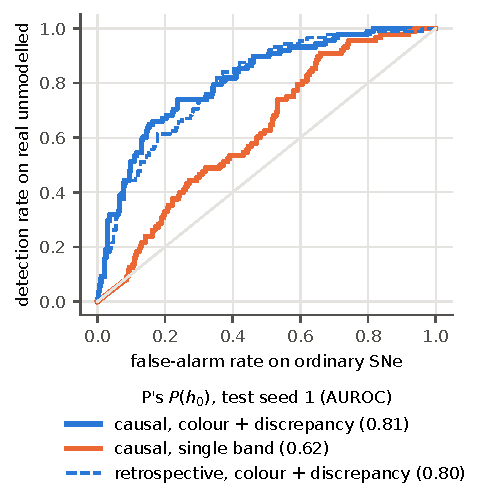
\includegraphics[width=\columnwidth]{fig4_roc_real.pdf}
\caption{Real data. How well $P(h_0)$ separates real unknown transients (TDE, SLSN, SN~Ibn) from ordinary supernovae. Colour plus a model-discrepancy term is what makes it work, and measuring only forward in time leaves the curve almost unchanged.}
\label{fig:rocreal}
\end{figure}

\paragraph{Time order changes the answer.} Our first version of this replay let planners go back and measure earlier epochs after later ones, which no spacecraft can do. Once we enforced the time arrow, the planners used far fewer measurements (P \RealCObsP\ of 5, against \RealRObsP\ before), because a one-step utility jumps to a late, informative epoch and gives up the earlier ones. With less data every posterior became less sure, so confident errors fell on both known and unknown events, and P's false ``unknown'' rate on supernovae fell from \RealRFaP\ to \RealCFaP. Two of our conclusions flipped from fail to pass just by respecting causality.


\section{Study 3: a guaranteed false-alarm rate}\label{sec:conf}
The Bayesian $h_0$ makes few confident errors, but it promises nothing about how often it cries ``unknown'' by mistake. So we added a second decision rule that does, and we tested it on supernovae nobody had used before.

\paragraph{Method.} After any planner's measurements $D$, we compute $s=\log p(D\mid h_0)-\max_c\log p(D\mid c)$ and flag ``unknown'' when $s$ goes above a threshold $\tau$. We set $\tau$ by split-conformal calibration on known supernovae, so if new supernovae look like the calibration ones, the chance of a false ``unknown'' is at most $\alpha=\ConfAlpha$, for any planner \citep{Vovk2005,Angelopoulos2023}. We also added a lookahead planner L, which gives some value ($\lambda=\ConfLambda$, chosen on validation data) to keeping later epochs available, because the greedy planner used too little of its budget. We drew \ConfNCal\ calibration and \ConfNFresh\ sealed test supernovae from Bright Transient Survey events that no earlier analysis had touched.

\begin{table*}[t]
\centering\scriptsize
\caption{Conformal open-set study, preregistered results per noise seed: estimate [95\% CI]; $^\times$ marks a criterion not met. Primary system: lookahead planner L with the conformal decision (C-L). $\Delta$: C-L minus closed-world EIG (B3), except HC6 (AUROC of $s$, L minus P). HC1 uses Clopper--Pearson intervals; HC2--HC4 and HC6 use the paired bootstrap.}
\label{tab:conf}
\begin{tabular}{llll}
\toprule
Hypothesis & Seed 1 & Seed 2 & Seed 3 \\
\midrule
HC1 false ``unknown'', sealed SNe ($\leq\alpha$) & +0.035 [+0.020, +0.055] & +0.061 [+0.042, +0.086] & +0.063 [+0.043, +0.089] \\
HC2 $\Delta$acc.\ SNe ($>-0.05$) & +0.082 [+0.039, +0.123] & +0.074 [+0.033, +0.115] & +0.059 [+0.012, +0.106] \\
HC3 $\Delta$CW SNe ($<+0.05$) & -0.027 [-0.057, +0.002] & -0.049 [-0.078, -0.020] & -0.012 [-0.043, +0.018] \\
HC4 $\Delta$CW unknowns ($<0$) & -0.239 [-0.375, -0.102] & -0.261 [-0.409, -0.114] & -0.193 [-0.341, -0.045] \\
HC5 unknowns flagged ($>\alpha$) & +0.420 [+0.316, +0.530] & +0.545 [+0.436, +0.652] & +0.432 [+0.327, +0.542] \\
HC6 $\Delta$AUROC, L$-$P ($>0$) & +0.012 [-0.013, +0.038]$^\times$ & +0.031 [+0.006, +0.058] & +0.039 [+0.005, +0.075] \\
\bottomrule
\end{tabular}

\end{table*}

\paragraph{The guarantee held, and accuracy went up.} On the sealed supernovae, the false-``unknown'' rate was \ConfFa, inside the promised \ConfAlphaPct. The lookahead planner with the conformal rule was also \ConfAccGain\ more accurate than closed-world information gain, which settles the cost question that Study~2 left open. On the real unknowns it flagged \ConfFlag. Lookahead did not, however, rank the unknowns any better than P did (Table~\ref{tab:conf}).

\paragraph{Two rules, two kinds of safety.} The conformal rule works on top of any planner, even a closed-world one, which then flagged \ConfFlagBthreeConf\ of the unknowns. But it is more often confidently wrong on unknowns (\ConfCwUnkCL\ against \ConfCwUnkP\ for P's Bayesian rule). So the conformal rule buys a certified false-alarm rate and accuracy on known classes, and the Bayesian $h_0$ buys fewer confident errors on the unknown.

\paragraph{A guarantee with no calibration at all.} The conformal rule still needs calibration events, so we also tried the e-process of Eq.~\eqref{eq:eprocess}, which needs none. We replayed every planner exactly, measurement for measurement, and raised ``unknown'' the first time $E_t$ reached 10. Real light curves never match a template exactly, so this was a real test of the guarantee. On the \EFreshN\ sealed supernovae, P's false-``unknown'' rate was only \EFreshFa\ against the promised 10\%, and it still caught \EDet\ of the \EWithheldN\ real unknowns. That is fewer than $P(h_0)$ catches (\RealCFlagP), but the guarantee now holds at every step. Because the test works on any planner, it caught even more on planners that measure more (\EDetL\ for lookahead), so a planner that ignores $h_0$ can still be given a safe ``unknown'' label afterwards.


\section{Study 4: a fleet that cannot always talk}\label{sec:fleet}

\paragraph{Setup.} Four transients go off at once, and eight satellites on real orbits share the work, each with three measurements to spend. We compare four fleets. In the ideal fleet (O) every satellite always hears every other. In the realistic fleets (A) satellites share and coordinate only when they are in line of sight, within a range $R$ of 1000 to 5000\,km. A third kind (K) shares data the same way but plans alone, and the last (G) never talks at all. Links turned out to be rare, so two satellites could talk only \FleetLinkUpOne--\FleetLinkUpFive\ of the time.

\paragraph{Talking helps, if the links are good.} With ideal links, the fleet was \FleetHFourOneMag\ percentage points more accurate than satellites working alone. Our first test with realistic links showed no gain, but that test was not fair, because the rule we had fixed for choosing how readily each fleet spends its measurements made the realistic fleet more frugal (\FleetObsA\ measurements per event against \FleetObsG). So we wrote new predictions and ran a second test on fresh events with equal spending, and then realistic links helped by \FleetBOneMag\ points. In both tests, coordinating plans added nothing once satellites shared what they had seen.

\begin{table*}[t]
\centering\tabularfont
\caption{Fleet test results (nominal, preregistered reserves). Acc.\ mod.: accuracy on modelled events (\%); CW unk.: confidently wrong on unknowns (\%); Flag unk.: unknowns labelled $h_0$ (\%); $\bar n_{\rm obs}$: measurements per event; Stale: share of already-taken records a spacecraft does not yet know (\%).}
\label{tab:fleet}
\begin{tabular}{lrrrrrrr}
\toprule
Strategy & Acc.\ mod. & CW unk. & Flag unk. & AUROC & log score & $\bar n_{\rm obs}$ & Stale \\
\midrule
Ideal links (oracle) & 87 & 8 & 48 & 0.93 & -0.80 & 5.1 & 0 \\
Auction, ISL $\leq$5000\,km & 75 & 0 & 45 & 0.90 & -0.88 & 3.7 & 29 \\
Knowledge only, ISL $\leq$5000\,km & 74 & 0 & 42 & 0.89 & -0.91 & 3.8 & 29 \\
Auction, ISL $\leq$1000\,km & 72 & 1 & 39 & 0.88 & -0.95 & 3.8 & 45 \\
No links & 76 & 4 & 39 & 0.88 & -0.99 & 5.4 & 88 \\
\bottomrule
\end{tabular}

\end{table*}

\begin{figure}[t]
\centering
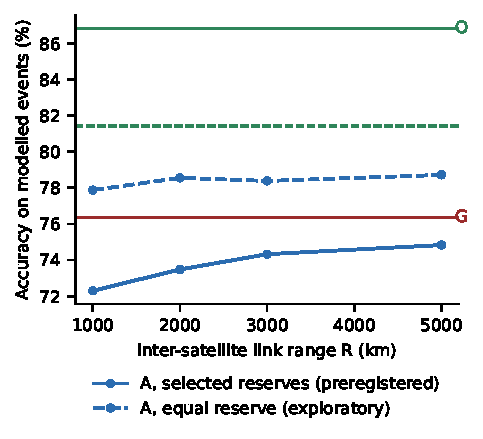
\includegraphics[width=\columnwidth]{fig5_fleet.pdf}
\caption{Fleet accuracy against how far satellites can talk. Horizontal lines are the ideal fleet (O, green) and satellites working alone (G, red). Solid lines use the spending rule fixed in advance, and dashed lines give every fleet the same rule.}
\label{fig:fleet}
\end{figure}

\paragraph{When to spend matters as much as talking.} Giving the ideal fleet a different spending rule alone moved its accuracy by \FleetBThreeMag\ points, about as much as perfect communication did (Fig.~\ref{fig:fleet}, Table~\ref{tab:fleet}).

\paragraph{Where the satellites sit matters most.} We expected a tightly packed fleet in one orbital plane to do well, because its satellites can talk far more (links up \FleetDenseLinkUpOne--\FleetDenseLinkUpFive\ of the time). Even with ideal links, it was \FleetBFourMag\ points less accurate than the spread-out fleet. Satellites in the same plane lose and regain sight of a target together, so they measure each event at fewer distinct times, and a fading transient is all about timing.

\paragraph{False alarms stay rare across the fleet.} Each satellite can also carry the e-process. It raised at most \FleetHEOneMaxK\ false ``unknown'' in \FleetHEOneN\ known events, and when satellites averaged the evidence they had heard from each other, there were \FleetHETwoK\ false alarms in \FleetHETwoN\ checks. When we deliberately gave every template the wrong timescale, the alarms rose to \FleetMEFalseUnknownO, which is the test doing its job, since the templates really were wrong.

\section{Discussion}\label{sec:disc}

\paragraph{The belief does the work.} The one finding that holds in every study is that keeping $h_0$ in the posterior stops confident misclassification of the unknown. The utility term built to test $h_0$ ($\beta$) made no measurable difference. In simulation, a closed-world entropy threshold on P's own measurements reached an AUROC of only \SimAucPown, against \SimAucP\ for $P(h_0)$ on the same measurements. So what makes the unknown recognisable is a hypothesis space that can name it, plus colour on real data. This goes against the intuition that a planner must hunt for anomalies. It first needs to be able to say ``none of these''.

\paragraph{Two kinds of guarantee.} The Bayesian $h_0$ made the fewest confident errors on real unknowns, but it promises nothing about false alarms. The conformal threshold gets a certified false-alarm rate from exchangeable calibration events, and that rate holds at the end of the budget. The e-process gets validity at every step and on any planner from the model itself, and we can average it across spacecraft whose data overlap. It pays in power, and in principle it is only as good as the templates, but on real supernovae that never match a template exactly it still stayed at \EFreshFa\ false alarms. So the choice depends on which error costs more, and on whether we trust the calibration set or the physics more.

\paragraph{The time arrow.} An earlier version of our pipeline let planners measure earlier epochs after later ones. This did not bias the comparison between strategies, but it changed the conclusions. Once measurements were causal, adaptive planners used about half of their budget, posteriors became less confident, and the supernova-cost hypothesis of Study~2 went from fail to pass. That is why we think benchmarks for follow-up planning should check the time order of every chosen sequence.

\paragraph{What a fleet needs.} Three things moved accuracy, and their order surprised us. Where the satellites are mattered most, since a spread fleet beat a single plane by \FleetBFourEst\ points. When they spend a measurement came next (\FleetBThreeEst). Whether they share what they have seen came last (\FleetBOneEst\ for realistic links and \FleetHFourOneEst\ for ideal ones). Coordinating plans added nothing in either test once knowledge was shared. So for small science fleets, we would invest in orbital diversity and in getting observations to each other, before negotiating who observes. CRDT sharing kept this safe, and no record was ever counted twice, whatever path it took.

\paragraph{What did not work.} Table~\ref{tab:tests} shows the failures next to the successes. The planner was not the fastest identifier, the urgency term hurt the fastest class, lookahead did not rank unknowns better, and realistic links only helped once spending was made equal. We report these as plainly as the rest, because they say where the method stops working.

\paragraph{Limitations.} Simulated light curves are analytic shapes, and amplitude is their only parameter. The decay term is a squared signal-to-noise proxy. There is no slew, exposure or link-budget model, and fleet links are purely geometric. On real data, we resample measurements from interpolated light curves and assume two-band imaging, and the test events were examined more than once, which we declared in advance. In the fleet study, two reserve prices sit at the edge of the validation grid, the satellites use old element sets, and the equal-reserve run in Study~4 is an extra look at the first test seed.

\section{Conclusion}\label{sec:concl}
For autonomous follow-up of fading transients, give the planner a way to say ``none of the above''. In simulation and on real ZTF events, this is the part of the method that keeps stopping confident misclassification of the unknown, and once measurements are causal it costs little on ordinary events. If a guaranteed false-alarm rate matters, a conformal threshold gives one at the end of the budget, and an e-process gives one at every step and across spacecraft without calibration data. A one-step utility does not manage urgency well, so we would not rely on it for that, and every follow-up study should check the time arrow. For a fleet, spread the satellites out, decide carefully when to spend, and share what you have seen before negotiating what to see next.

\section*{Acknowledgements}
We thank Dr.\ Ambedkar Institute of Technology, Bengaluru, for its continuous support of this work.

\section*{Declarations}

\begin{itemize}
\item Funding: Not applicable. This research received no external funding.
\item Competing interests: None.
\item Data availability: ZTF Bright Transient Survey light curves are public. Every per-event result, preregistration file and the scripts that generate every number, table and figure in this paper are in the code repository below.
\item Code availability: \url{https://github.com/joycemalik/orbitalnet-dashboard}, branch \texttt{research/open-world-planner}.
\item Author contributions: All authors (J.M., A.H., M.B., S.S., S.S.B. and H.G.) contributed to the conception and design of the framework and to the writing of the manuscript. All authors read and approved the final manuscript.
\end{itemize}

\bibliography{refs}

\end{document}
